% -*- TeX-engine: xetex; eval: (auto-fill-mode 0); eval: (visual-line-mode 1); -*-
% Compile with XeLaTeX

%%%%%%%%%%%%%%%%%%%%%%%
% Option 1: Slides: (comment for handouts)   %
%%%%%%%%%%%%%%%%%%%%%%%

%\documentclass[slidestop,compress,mathserif,12pt,t,professionalfonts,xcolor=table]{beamer}
%
%% solution stuff
%\newcommand{\solnMult}[1]{
%\only<1>{#1}
%\only<2->{\red{\textbf{#1}}}
%}
%\newcommand{\soln}[1]{\textit{#1}}

%%%%%%%%%%%%%%%%%%%%%%%%%%%%%%%
% Option 2: Handouts, without solutions (post before class)    %
%%%%%%%%%%%%%%%%%%%%%%%%%%%%%%%

 \documentclass[11pt,containsverbatim,handout,xcolor=xelatex,dvipsnames,table]{beamer}

 % handout layout
 \usepackage{pgfpages}
 \pgfpagesuselayout{4 on 1}[letterpaper,landscape,border shrink=5mm]

 % solution stuff
 \newcommand{\solnMult}[1]{#1}
 \newcommand{\soln}[1]{}

%%%%%%%%%%%%%%%%%%%%%%%%%%%%%%%%%%%%
% Option 3: Handouts, with solutions (may post after class if need be)    %
%%%%%%%%%%%%%%%%%%%%%%%%%%%%%%%%%%%%

% \documentclass[11pt,containsverbatim,handout,xcolor=xelatex,dvipsnames,table]{beamer}

% % handout layout
% \usepackage{pgfpages}
% \pgfpagesuselayout{4 on 1}[letterpaper,landscape,border shrink=5mm]

% % solution stuff
% \newcommand{\solnMult}[1]{\red{\textbf{#1}}}
% \newcommand{\soln}[1]{\textit{#1}}

%%%%%%%%%%
% Load style file, defaults  %
%%%%%%%%%%

%%%%%%%%%%%%%%%%
% Themes
%%%%%%%%%%%%%%%%

% See http://deic.uab.es/~iblanes/beamer_gallery/ for mor options

% Style theme
\usetheme{Pittsburgh}

% Color theme
\usecolortheme{seahorse}

% Helvetica Neue Light for most text
\usepackage{fontspec}
\setsansfont{Helvetica Neue Light}

%%%%%%%%%%%%%%%%
% Packages
%%%%%%%%%%%%%%%%

\usepackage{geometry}
\usepackage{graphicx}
\usepackage{amssymb}
\usepackage{epstopdf}
\usepackage{amsmath}  	% this permits text in eqnarray among other benefits
\usepackage{url}		% produces hyperlinks
\usepackage[english]{babel}
\usepackage{colortbl}	% allows for color usage in tables
\usepackage{multirow}	% allows for rows that span multiple rows in tables
\usepackage{color}		% this package has a variety of color options
\usepackage{pgf}
\usepackage{calc}
\usepackage{ulem}
\usepackage{multicol}
\usepackage{textcomp}
\usepackage{listings}
\usepackage{changepage}
\usepackage{tikz}
\usetikzlibrary{trees}		% for probability trees
\usepackage{fancyvrb}	% for colored code chunks
\usepackage{nameref}

%%%%%%%%%%%%%%%%
% Remove navigation symbols
%%%%%%%%%%%%%%%%

\beamertemplatenavigationsymbolsempty
\hypersetup{pdfpagemode=UseNone} % don't show bookmarks on initial view

%%%%%%%%%%%%%%%%
% User defined colors
%%%%%%%%%%%%%%%%

% Pantone 2016 Spring colors
% https://atelierbram.github.io/c-tiles16/colorscheming/pantone-spring-2016-colortable.html
% update each semester or year

\xdefinecolor{custom_blue}{rgb}{0.01, 0.31, 0.52} % Snorkel Blue
\xdefinecolor{custom_darkBlue}{rgb}{0.20, 0.20, 0.39} % Reflecting Pond  
\xdefinecolor{custom_orange}{rgb}{0.96, 0.57, 0.42} % Cadmium Orange
\xdefinecolor{custom_green}{rgb}{0, 0.47, 0.52} % Biscay Bay
\xdefinecolor{custom_red}{rgb}{0.58, 0.32, 0.32} % Marsala

\xdefinecolor{custom_lightGray}{rgb}{0.78, 0.80, 0.80} % Glacier Gray
\xdefinecolor{custom_darkGray}{rgb}{0.35, 0.39, 0.43} % Stormy Weather

%%%%%%%%%%%%%%%%
% Template colors
%%%%%%%%%%%%%%%%

\setbeamercolor*{palette primary}{fg=white,bg= custom_blue}
\setbeamercolor*{palette secondary}{fg=black,bg= custom_blue!80!black}
\setbeamercolor*{palette tertiary}{fg=white,bg= custom_blue!80!black!80}
\setbeamercolor*{palette quaternary}{fg=white,bg= custom_blue}

\setbeamercolor{structure}{fg= custom_blue}
\setbeamercolor{frametitle}{bg= custom_blue!90}
\setbeamertemplate{blocks}[shadow=false]
\setbeamersize{text margin left=2em,text margin right=2em}

%%%%%%%%%%%%%%%%
% Styling fonts, bullets, etc.
%%%%%%%%%%%%%%%%

% title slide
\setbeamerfont{title}{size=\large,series=\bfseries}
\setbeamerfont{subtitle}{size=\large,series=\mdseries}
%\setbeamerfont{institute}{size=\large,series=\mdseries}

% color of alerted text
\setbeamercolor{alerted text}{fg=custom_orange}

% styling of itemize bullets
\setbeamercolor{item}{fg=custom_blue}
\setbeamertemplate{itemize item}{{{\small$\blacktriangleright$}}}
\setbeamercolor{subitem}{fg=custom_blue}
\setbeamertemplate{itemize subitem}{{\textendash}}
\setbeamerfont{itemize/enumerate subbody}{size=\footnotesize}
\setbeamerfont{itemize/enumerate subitem}{size=\footnotesize}

% styling of enumerate bullets
\setbeamertemplate{enumerate item}{\insertenumlabel.}
\setbeamerfont{enumerate item}{family={\fontspec{Helvetica Neue}}}
\setbeamerfont{enumerate subitem}{family={\fontspec{Helvetica Neue}}}
\setbeamerfont{enumerate subsubitem}{family={\fontspec{Helvetica Neue}}}

% make frame titles small to make room in the slide
\setbeamerfont{frametitle}{size=\small} 

% set Helvetica Neue font for frame and section titles
\setbeamerfont{frametitle}{family={\fontspec{Helvetica Neue}}}
\setbeamerfont{sectiontitle}{family={\fontspec{Helvetica Neue}}}
\setbeamerfont{section in toc}{family={\fontspec{Helvetica Neue}}}
\setbeamerfont{subsection in toc}{family={\fontspec{Helvetica Neue}}, size=\small}
\setbeamerfont{footline}{family={\fontspec{Helvetica Neue}}}
\setbeamerfont{subsection in toc}{family={\fontspec{Helvetica Neue}}}
\setbeamerfont{block title}{family={\fontspec{Helvetica Neue}}}

%%%%%%%%%%%%%%%%
% New fonts accessed by fontspec package
%%%%%%%%%%%%%%%%

% Monaco font for code
\newfontfamily{\monaco}{Monaco}

%%%%%%%%%%%%%%%%
% Color text commands
%%%%%%%%%%%%%%%%

%orange
\newcommand{\orange}[1]{\textit{\textcolor{custom_orange}{#1}}}

% yellow
\newcommand{\yellow}[1]{\textit{\textcolor{yellow}{#1}}}

% blue
\newcommand{\blue}[1]{\textit{\textcolor{blue}{#1}}}

% green
\newcommand{\green}[1]{\textit{\textcolor{custom_green}{#1}}}

% red
\newcommand{\red}[1]{\textit{\textcolor{custom_red}{#1}}}

% dark gray
\newcommand{\darkgray}[1]{\textit{\textcolor{custom_darkGray}{#1}}}

% light gray
\newcommand{\lightgray}[1]{\textit{\textcolor{custom_lightGray}{#1}}}

% pink
\newcommand{\pink}[1]{\textit{\textcolor{pink}{#1}}}


%%%%%%%%%%%%%%%%
% Custom commands
%%%%%%%%%%%%%%%%

% empty box for probability tree frame
\newcommand{\emptybox}[2]{
	\fbox{ \begin{minipage}{#1} \hfill\vspace{#2} \end{minipage} }
}

% cancel
\newcommand{\cancel}[1]{%
    \tikz[baseline=(tocancel.base)]{
        \node[inner sep=0pt,outer sep=0pt] (tocancel) {#1};
        \draw[red, line width=0.5mm] (tocancel.south west) -- (tocancel.north east);
    }%
}

% degree
\newcommand{\degree}{\ensuremath{^\circ}}

% cite
\newcommand{\ct}[1]{
\vfill
{\tiny #1}}

% Note
\newcommand{\Note}[1]{
\rule{2.5cm}{0.25pt} \\ \textit{\footnotesize{\textcolor{custom_red}{Note:} \textcolor{custom_darkGray}{#1}}}}

% Remember
\newcommand{\Remember}[1]{\textit{\scriptsize{\textcolor{custom_red}{Remember:} #1}}}

% links: webURL, webLink
\newcommand{\webURL}[1]{\urlstyle{same}{\textit{\textcolor{custom_blue}{\url{#1}}}}}
\newcommand{\webLink}[2]{\href{#1}{\textcolor{custom_blue}{{#2}}}}

% mail
\newcommand{\mail}[1]{\href{mailto:#1}{\textit{\textcolor{custom_blue}{#1}}}}

% highlighting: hl, hlGr, mathhl
\newcommand{\hl}[1]{\textit{\textcolor{custom_blue}{#1}}}
\newcommand{\hlGr}[1]{\textit{\textcolor{custom_green}{#1}}}
\newcommand{\mathhl}[1]{\textcolor{custom_blue}{\ensuremath{#1}}}

% example
\newcommand{\ex}[1]{\textcolor{blue}{{{\small (#1)}}}}

% twocol: two columns
\newenvironment{twocol}[4]{
\begin{columns}[c]
\column{#1\textwidth}
#3
\column{#2\textwidth}
#4
\end{columns}
}

% threecol: three columns
\newenvironment{threecol}[6]{
\begin{columns}[c]
\column{#1\textwidth}
#4
\column{#2\textwidth}
#5
\column{#3\textwidth}
#6
\end{columns}
}

% slot (for probability calculations)
\newenvironment{slot}[2]{
\begin{array}{c} 
\underline{#1} \\ 
#2
\end{array}
}

% pr: left and right parentheses
\newcommand{\pr}[1]{
\left( #1 \right)
}

%%%%%%%%%%%%%%%%
% Custom blocks
%%%%%%%%%%%%%%%%

% activity: less commonly used
\newcommand{\activity}[2]{
\setbeamertemplate{itemize item}{{{\small\textcolor{custom_orange}{$\blacktriangleright$}}}}
\setbeamercolor{block title}{fg=white, bg=custom_orange}
\setbeamerfont{block title}{size=\small}
\setbeamercolor{block body}{fg=black, bg=custom_orange!20!white!80}
\setbeamerfont{block body}{size=\small}
\begin{block}{Activity: #1}
\setlength\abovedisplayskip{0pt}
#2
\end{block}
}

% app: application exercise
\newcommand{\app}[2]{
\setbeamercolor{block title}{fg=white,bg=custom_green}
\setbeamercolor{block body}{fg=black,bg=custom_green!20!white!80}
\begin{block}{{\small Application exercise: #1}}
#2
\end{block}
}

% disc: discussion question
\newcommand{\disc}[1]{
\vspace*{-2ex}
\setbeamercolor{block body}{bg=custom_blue!25!white!80, fg=custom_blue!55!black!95}
\begin{block}{\vspace*{-3ex}}
#1
\end{block}
\vspace*{-1ex}
}

% clicker: clicker question
\newcommand{\clicker}[1]{
\setbeamercolor{block title}{bg=custom_blue!80!white!50,fg=custom_blue!30!black!90}
\setbeamercolor{block body}{bg=custom_blue!20!white!80,fg=custom_blue!30!black!90}
\begin{block}{\vspace*{-0.2ex}{\footnotesize Clicker question}\vspace*{-0.2ex}}
#1
\end{block}
}

% formula
\newcommand{\formula}[2]{
\setbeamercolor{block title}{bg=custom_blue!40!white!60,fg=custom_blue!55!black!95}
\begin{block}{{\small#1}}
#2
\end{block}
}

% code
\newcommand{\Rcode}[1]{
{\monaco {\footnotesize \textcolor{custom_darkBlue}{#1}}}
}

% output
\newcommand{\Rout}[1]{
{\monaco {\footnotesize \textcolor{custom_darkGray}{#1}}}
}

%%%%%%%%%%%%%%%%
% Change margin
%%%%%%%%%%%%%%%%

\newenvironment{changemargin}[2]{%
\begin{list}{}{%
\setlength{\topsep}{0pt}%
\setlength{\leftmargin}{#1}%
\setlength{\rightmargin}{#2}%
\setlength{\listparindent}{\parindent}%
\setlength{\itemindent}{\parindent}%
\setlength{\parsep}{\parskip}%
}%
\item}{\end{list}}

%%%%%%%%%%%%%%%%
% Footnote
%%%%%%%%%%%%%%%%

\long\def\symbolfootnote[#1]#2{\begingroup%
\def\thefootnote{\fnsymbol{footnote}}\footnote[#1]{#2}\endgroup}

%%%%%%%%%%%%%%%%
% Graphics
%%%%%%%%%%%%%%%%

\DeclareGraphicsRule{.tif}{png}{.png}{`convert #1 `dirname #1`/`basename #1 .tif`.png}

%%%%%%%%%%%%%%%%
% Slide number
%%%%%%%%%%%%%%%%

\setbeamertemplate{footline}{%
    \raisebox{5pt}{\makebox[\paperwidth]{\hfill\makebox[20pt]{\color{gray}
          \scriptsize\insertframenumber}}}\hspace*{5pt}}

          
%%%%%%%%%%%%%%%%
% Remove page numbers
%%%%%%%%%%%%%%%%

\newcommand{\removepagenumbers}{% 
  \setbeamertemplate{footline}{}
}

%%%%%%%%%%%%%%%%
% TOC slides
%%%%%%%%%%%%%%%%

\setbeamertemplate{section in toc}{\inserttocsectionnumber.~\inserttocsection}
\setbeamertemplate{subsection in toc}{$\qquad$\inserttocsubsectionnumber.~\inserttocsubsection \\}

\AtBeginSection[] 
{ 
  \addtocounter{framenumber}{-1} 
  % 
  {\removepagenumbers 
  {\small
    \begin{frame}<beamer> 
    \frametitle{Outline} 
    \tableofcontents[currentsection] 
  \end{frame} 
  } 
  }
} 

\AtBeginSubsection[] 
{ 
  \addtocounter{framenumber}{-1} 
  % 
  {\removepagenumbers 
  {\small
    \begin{frame}<beamer> 
    \frametitle{Outline} 
    \tableofcontents[currentsection,currentsubsection] 
  \end{frame} 
  } 
  }
}
% Course Name
\newcommand{\CourseName}{Sta 101 - Spring 2016}
\newcommand{\InstituteName}{Duke University, Department of Statistical Science}

% Personal Info
\newcommand{\FirstName}{Mine}
\newcommand{\LastName}{\c{C}etinkaya-Rundel}

% Electronic Info
\newcommand{\PersonalSite}{http://stat.duke.edu/~mc301}
\newcommand{\CourseSite}{http://bit.ly/sta101_s16}
\newcommand{\Email}{mine@stat.duke.edu}

% Exam Dates
\newcommand{\ExamADate}{Feb 24, Wed}
\newcommand{\ExamBDate}{Mar 30, Wed}
\newcommand{\FinalDate}{May 5, Thu - 7-10pm}
% ALT ALT
% % Course Name
\newcommand{\CourseName}{Sta 101 - Spring 2016}
\newcommand{\InstituteName}{Duke University, Department of Statistical Science}

% Personal Info
\newcommand{\FirstName}{Anthea}
\newcommand{\LastName}{Monod}

% Electronic Info
\newcommand{\PersonalSite}{https://stat.duke.edu/people/anthea-monod.html}
\newcommand{\CourseSite}{https://stat.duke.edu/courses/Spring16/sta101.002}
\newcommand{\Email}{anthea@stat.duke.edu}

% Exam Dates
\newcommand{\ExamADate}{Feb 25, Thu}
\newcommand{\ExamBDate}{Mar 31, Thu}
\newcommand{\FinalDate}{???}

%%%%%%%%%%%
% Cover slide info    %
%%%%%%%%%%%

\title{Unit 3: Foundations for inference}
\subtitle{1. Variability in estimates and CLT}
\author{\CourseName}
\date{}
\institute{\InstituteName}


%%%%%%%%%%%%%%%%%%%%%%%%%
% Begin document and set Helvetica Neue font   %
%%%%%%%%%%%%%%%%%%%%%%%%%

\begin{document}
\fontspec[Ligatures=TeX]{Helvetica Neue Light}

%%%%%%%%%%%%%%%%%%%%%%%%%%%%%%%%%%%

% Title Page

\begin{frame}[plain]

\titlepage

\vfill

{\scriptsize \webLink{\PersonalSite}{Dr. \LastName{}} \hfill Slides posted at  \webURL{\CourseSite}}

\addtocounter{framenumber}{-1} 

\end{frame}

%%%%%%%%%%%%%%%%%%%%%%%%%%%%%%%%%%%%

\section{Housekeeping}

%%%%%%%%%%%%%%%%%%%%%%%%%%%%%%%%%%%%

\begin{frame}
\frametitle{Announcements}

\begin{itemize}

\item My Thursday OH moved to 1-2:30pm on Sunday

\item If I asked to meet with your team, and you have not yet signed up for a time slot, please come to my Sunday office hours

\end{itemize}

\end{frame}

%%%%%%%%%%%%%%%%%%%%%%%%%%%%%%%%%%%%

\section{Main ideas}

%%%%%%%%%%%%%%%%%%%%%%%%%%%%%%%%%%%%

\subsection{Sample statistics vary from sample to sample}
\label{mi1}

%%%%%%%%%%%%%%%%%%%%%%%%%%%%%%%%%%%%

\begin{frame}
\frametitle{Sample statistics vary from sample to sample}

\begin{itemize}

\item We are often interested in \hl{population parameters}.

\item Since complete populations are difficult (or impossible) to collect data on, we use \hl{sample statistics} as \hl{point estimates} for the unknown population parameters of interest.

\item Sample statistics vary from sample to sample.

\item Quantifying how sample statistics vary provides a way to estimate the \hl{margin of error} associated with our point estimate.

\item But before we get to quantifying the variability among samples, let's try to understand how and why point estimates vary from sample to sample.

\end{itemize}

\disc{Suppose we randomly sample 1,000 adults from each state in the US. Would you expect the sample means of their ages to be the same, somewhat different, or very different?}

\end{frame}

%%%%%%%%%%%%%%%%%%%%%%%%%%%%%%%%%%%

\begin{frame}
\frametitle{}

\disc{We would like to estimate the average number of drinks it takes students to get drunk. 
\begin{itemize}
\item We will assume that our population is comprised of 146 students.
\item Assume also that we don't have the resources to collect data from all 146, so we will take a sample of size $n = 10$. 
\end{itemize}
If we randomly select observations from this data set, which values are most likely to be selected, which are least likely?}

\begin{center}
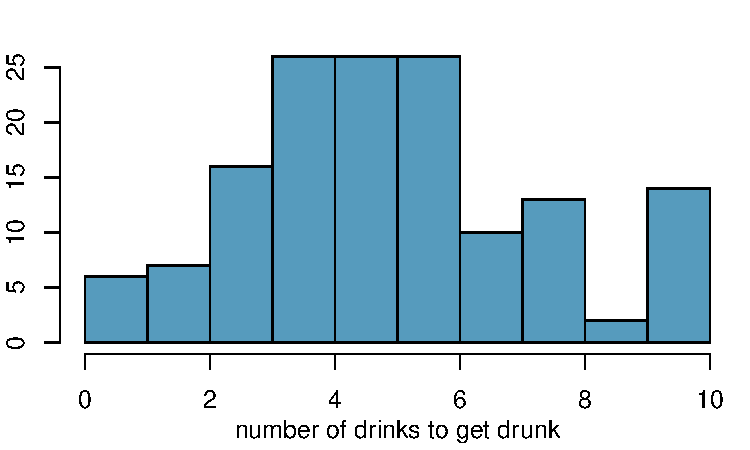
\includegraphics[width=0.6\textwidth]{figures/no_drinks_drunk/hist_no_drinks_drunk_pop} 
\end{center}

\end{frame}

%%%%%%%%%%%%%%%%%%%%%%%%%%%%%%%%%%%

\begin{frame}[fragile]
\frametitle{}

\begin{itemize}

\item Sample, with replacement, ten student IDs:
{\footnotesize
\begin{Verbatim}[frame=single, formatcom=\color{blue}]
> sample(1:146, size = 10, replace = TRUE)
\end{Verbatim}
}
\pause
{\footnotesize
\begin{Verbatim}[frame=single, formatcom=\color{gray}]
[1]  59 121  88  46  58  72  82  81   5  10
\end{Verbatim}
}
\pause

\item Find the students with these IDs:

\begin{center}
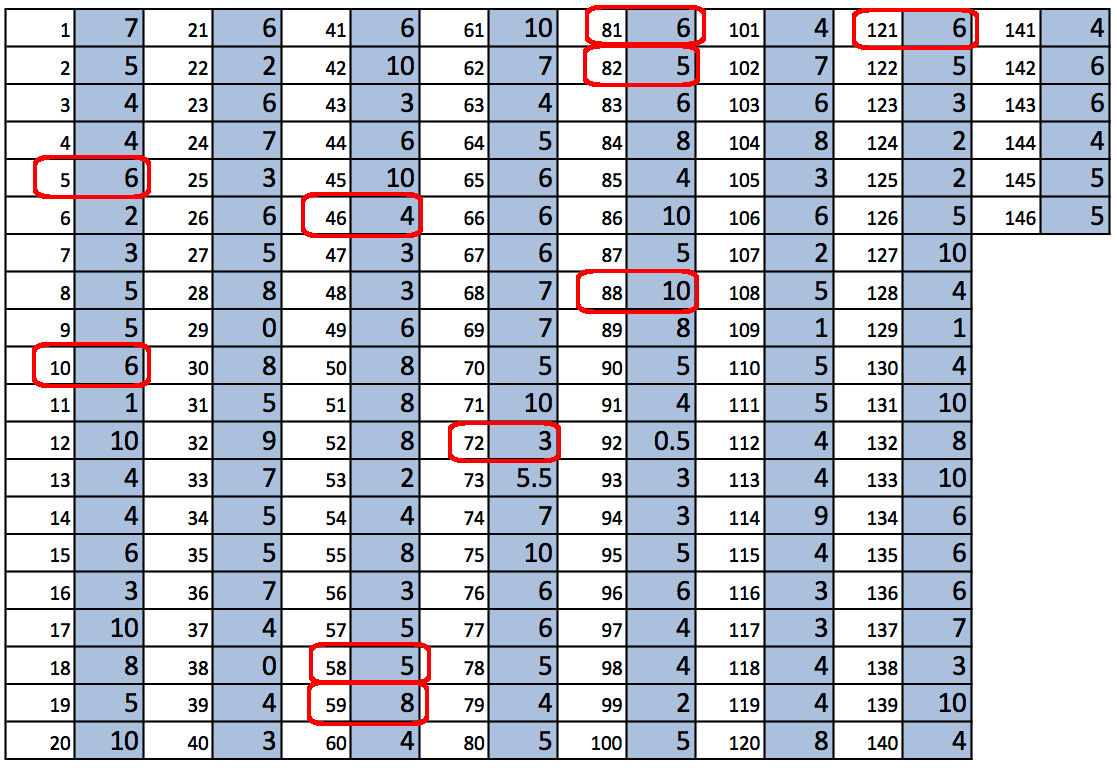
\includegraphics[width=0.65\textwidth]{figures/no_drinks_drunk/no_drinks_drunk_mysample}
\end{center}

\pause

\item Calculate the sample mean: $(8+6+10+4+5+3+5+6+6+6) / 10 = 5.9$

\end{itemize}

\end{frame}

%%%%%%%%%%%%%%%%%%%%%%%%%%%%%%%%%%%%

\begin{frame}[fragile]
\frametitle{}

\activity{Creating a sampling distribution}{Repeat this in teams, and report your sample mean.}
\begin{enumerate}

\item Sample, with replacement, ten student IDs:
{\footnotesize
\begin{Verbatim}[frame=single, formatcom=\color{blue}]
> sample(1:146, size = 10, replace = TRUE)
\end{Verbatim}
}

\item Find the students with these IDs:

\begin{center}
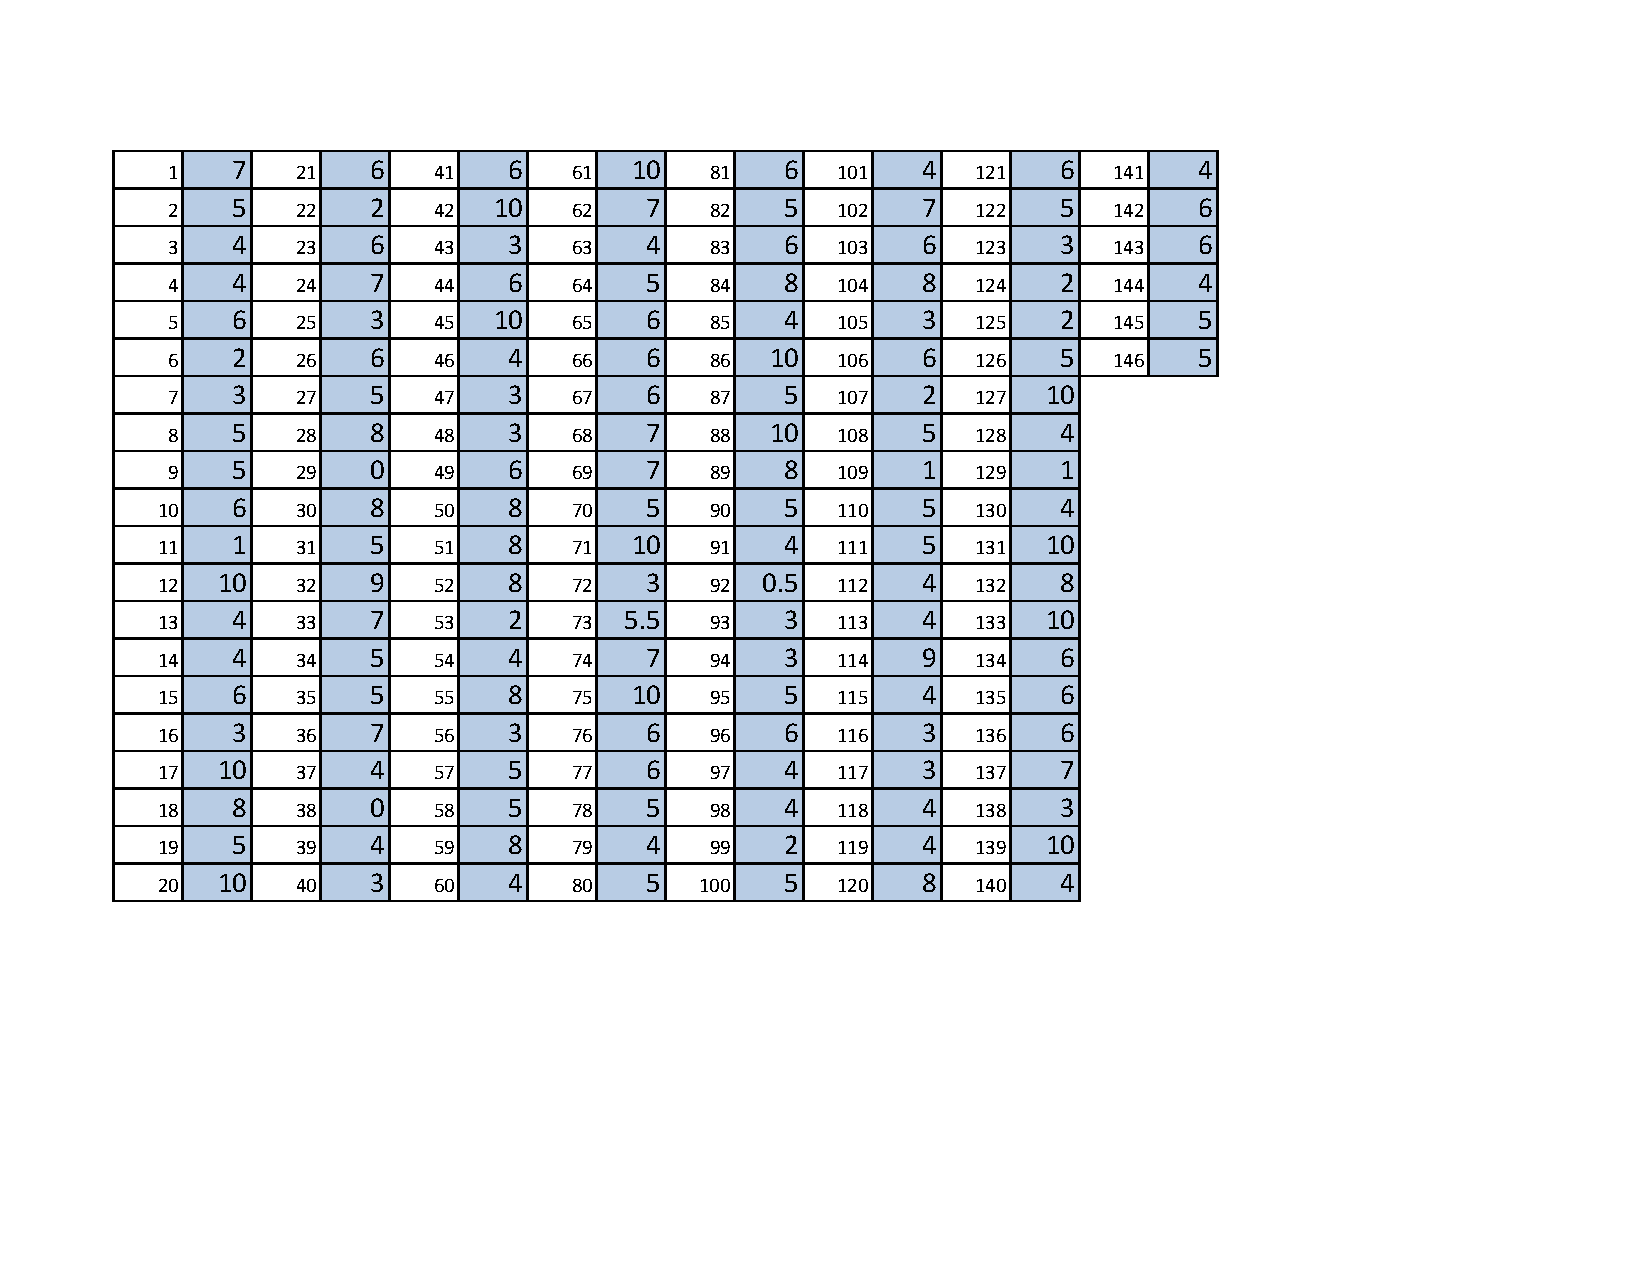
\includegraphics[width=0.6\textwidth]{figures/no_drinks_drunk/no_drinks_drunk_clean}
\end{center}

\item Calculate the sample mean, round it to 2 decimal places, and submit it using your clicker. Submit once per sample!

\end{enumerate}

\end{frame}

%%%%%%%%%%%%%%%%%%%%%%%%%%%%%%%%%%%

\begin{frame}[fragile]
\frametitle{Sampling distribution}

What you just constructed is called a \hl{sampling distribution}.

$\:$ \\
\disc{What is the shape and center of this distribution. Based on this distribution what do you think is the true population average?}

$\:$ \\
\soln{\only<2>{
5.39
}}

\end{frame}


%%%%%%%%%%%%%%%%%%%%%%%%%%%%%%%%%%%%

\begin{frame}[fragile]
\frametitle{Average number of Duke games attended}

Next let's look at the population data for the number of Duke basketball games attended:

\begin{center}
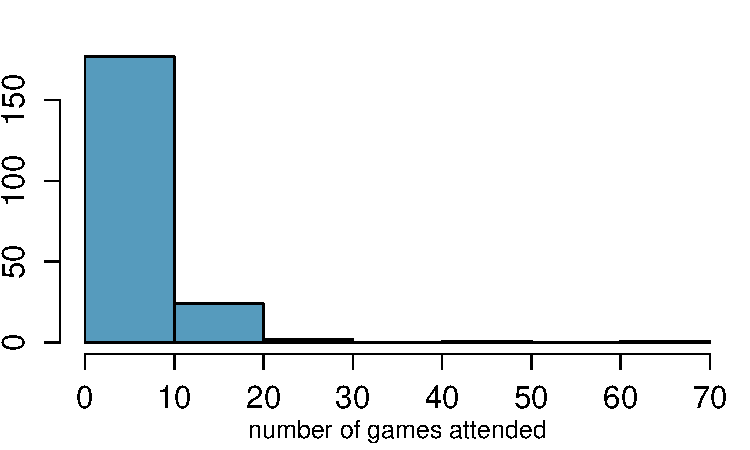
\includegraphics[width=0.8\textwidth]{figures/duke_games/hist_duke_games_pop}
\end{center}


\end{frame}

%%%%%%%%%%%%%%%%%%%%%%%%%%%%%%%%%%%%

\begin{frame}[fragile]
\frametitle{Average number of Duke games attended (cont.)}

Sampling distribution, n = 10:

\twocol{0.6}{0.4}{
\begin{center}
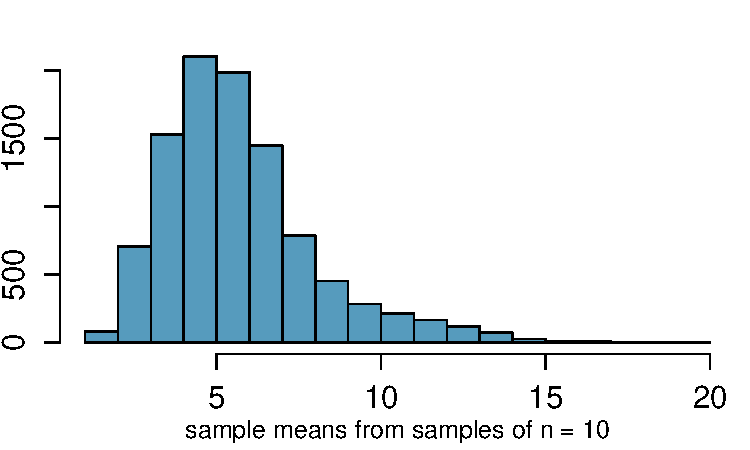
\includegraphics[width=\textwidth]{figures/duke_games/hist_duke_games_sampling10}
\end{center}
}
{
\disc{What does each observation in this distribution represent?}
\soln{\only<2->{Sample mean, $\bar{x}$, of samples of size $n = 10$.}}
\disc{Is the variability of the sampling distribution smaller or larger than the variability of the population distribution?}
\soln{\only<3->{Smaller, sample means will vary less than individual observations.}}
}

\end{frame}

%%%%%%%%%%%%%%%%%%%%%%%%%%%%%%%%%%%%

\begin{frame}[fragile]
\frametitle{Average number of Duke games attended (cont.)}

Sampling distribution, n = 30:

\twocol{0.6}{0.4}{
\begin{center}
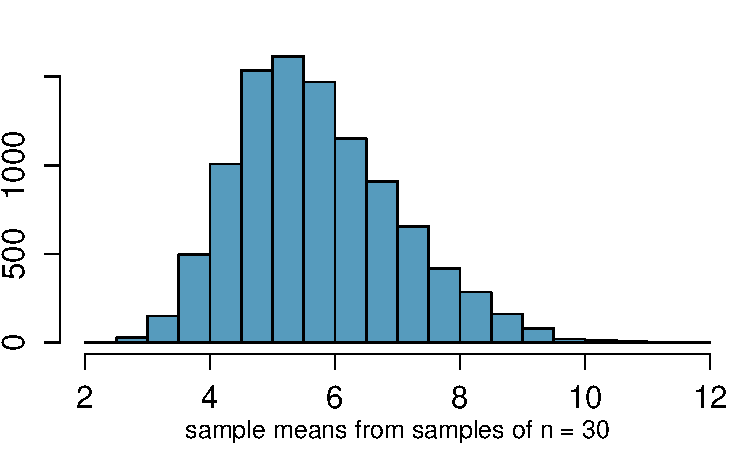
\includegraphics[width=\textwidth]{figures/duke_games/hist_duke_games_sampling30}
\end{center}
}
{
\disc{How did the shape, center, and spread of the sampling distribution change going from $n = 10$ to $n = 30$?}
\soln{\only<2->{Shape is more symmetric, center is about the same, spread is smaller.}}
}

\end{frame}

%%%%%%%%%%%%%%%%%%%%%%%%%%%%%%%%%%%%

\begin{frame}[fragile]
\frametitle{Average number of Duke games attended (cont.)}

Sampling distribution, n = 70:

\begin{center}
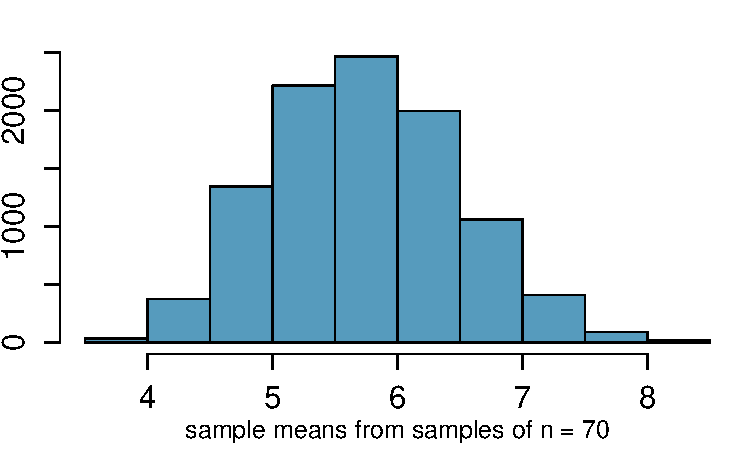
\includegraphics[width=0.6\textwidth]{figures/duke_games/hist_duke_games_sampling70}
\end{center}

\end{frame}

%%%%%%%%%%%%%%%%%%%%%%%%%%%%%%%%%%%%

\begin{frame}[fragile]
\frametitle{Average number of Duke games attended (cont.)}

\clicker{The mean of the sampling distribution is 5.75, and the standard deviation of the sampling distribution (also called the \hl{standard error}) is 0.75. Which of the following is the most reasonable guess for the 95\% confidence interval for the true average number of Duke games attended by students?}

\begin{enumerate}[(a)]
\item $5.75 \pm 0.75$
\item \solnMult{$5.75 \pm 2 \times 0.75$} \soln{\only<2>{\red{$\rightarrow (4.25,7.25)$}}}
\item $5.75 \pm 3 \times 0.75$
\item cannot tell from the information given
\end{enumerate}

\end{frame}

%%%%%%%%%%%%%%%%%%%%%%%%%%%%%%%%%%%%

\subsection{CLT describes the shape, center, and spread of sampling distributions}
\label{mi2}

%%%%%%%%%%%%%%%%%%%%%%%%%%%%%%%%%%%%

\begin{frame}
\frametitle{2. CLT describes the shape, center, and spread of sampling distributions}

\emph{Under the right conditions}, the distribution of the sample means is well
approximated by a normal distribution:
\[ \bar{x} \sim N \pr{ mean = \mu, SE = \frac{\sigma}{\sqrt{n}} } \]
A cheat: If $\sigma$ is unknown, use $s$.

\pause

\begin{itemize}

\item So it wasn't a coincidence that the sampling distributions we saw earlier were symmetric.

\item We won't go into the proving why $SE =  \frac{\sigma}{\sqrt{n}}$, but note that as $n$ increases $SE$ decreases. 

\item As the sample size increases we would expect samples to yield more consistent sample means, hence the variability among the sample means would be lower.

\end{itemize}

\end{frame}

%%%%%%%%%%%%%%%%%%%%%%%%%%%%%%%%%%%%

\subsection{CLT only applies when independence and sample size/skew conditions are met}
\label{mi3}

%%%%%%%%%%%%%%%%%%%%%%%%%%%%%%%%%%%%

\begin{frame}
\frametitle{3. CLT only applies when independence and sample size/skew conditions are met}

\begin{enumerate}

\item \hlGr{Independence:} Sampled observations must be independent. \\

$\:$ \\
This is difficult to verify, but is more likely if
\begin{itemize}
\item random sampling/assignment is used, and,
\item if sampling without replacement, $n$ $<$ 10\% of the population.
\end{itemize}

\pause

\item \hlGr{Sample size/skew:} Either 

\begin{itemize}
\item the population distribution is normal or
\item $n > 30$ and the population dist.\ is not extremely skewed, or
\item $n >> 30$ (approx.\ gets better as $n$ increases).
\end{itemize}

This is also difficult to verify for the population, but we can check it using the sample data, and assume that the sample mirrors the population.

\end{enumerate}

\end{frame}

%%%%%%%%%%%%%%%%%%%%%%%%%%%%%%%%%%%%

\begin{frame}
\frametitle{3. CLT only applies when independence and sample size/skew conditions are met}

Amongst other things, the central limit theorem is useful for 
\begin{itemize}
\item constructing confidence intervals and
\item conducting hypothesis tests.
\end{itemize}

\end{frame}

%%%%%%%%%%%%%%%%%%%%%%%%%%%%%%%%%%%%

\begin{frame}
\frametitle{}

\clicker{Which of the below visualizations is \emph{not} appropriate for checking the shape of the sample distribution of a numerical variable, and hence the population?}

\begin{enumerate}[(a)]
\item histogram
\item boxplot
\item normal probability plot
\item \solnMult{mosaicplot}
\end{enumerate}

\end{frame}

%%%%%%%%%%%%%%%%%%%%%%%%%%%%%%%%%%%%

\section{Summary}

%%%%%%%%%%%%%%%%%%%%%%%%%%%%%%%%%%%%

\begin{frame}
\frametitle{Summary of main ideas}

\vfill

\begin{enumerate}

\item \nameref{mi1}

\item \nameref{mi2}

\item \nameref{mi3}

\end{enumerate}

\vfill

\end{frame}

%%%%%%%%%%%%%%%%%%%%%%%%%%%%%%%%%%%

\section{Exercises [time permitting]}

%%%%%%%%%%%%%%%%%%%%%%%%%%%%%%%%%%%

\begin{frame}
\frametitle{}

\clicker{
{\footnotesize Four plots: Determine which plot (A, B, or C) is which. \\
(1) At top: distribution for a population ($\mu = 60, \sigma = 18$), \\
(2) a single random sample of 500 observations from this population, \\
(3) a distribution of 500 sample means from random samples with size 18,  \\
(4) a distribution of 500 sample means from random samples with size 81.}}

\twocol{0.4}{0.6}{
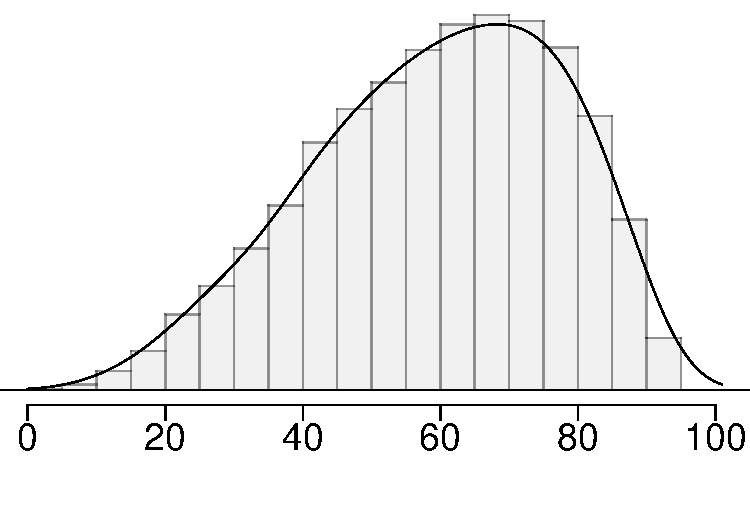
\includegraphics[width=\textwidth]{figures/cltSimLS/cltSimLS_pop}
}
{
\vspace{-0.5cm}
{\small
\begin{enumerate}[(a)]
\item (2) - B; (3) - A; (4) - C
\item (2) - A; (3) - B; (4) - C
\item (2) - C; (3) - A; (4) - D
\item \solnMult{(2) - B; (3) - C; (4) - A}
\end{enumerate}
}
}
\vspace{-0.25cm}
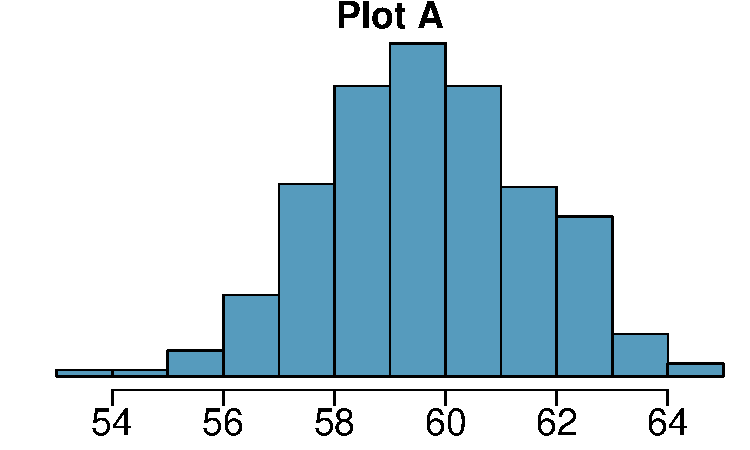
\includegraphics[width=0.32\textwidth]{figures/cltSimLS/cltSimLS_n81}
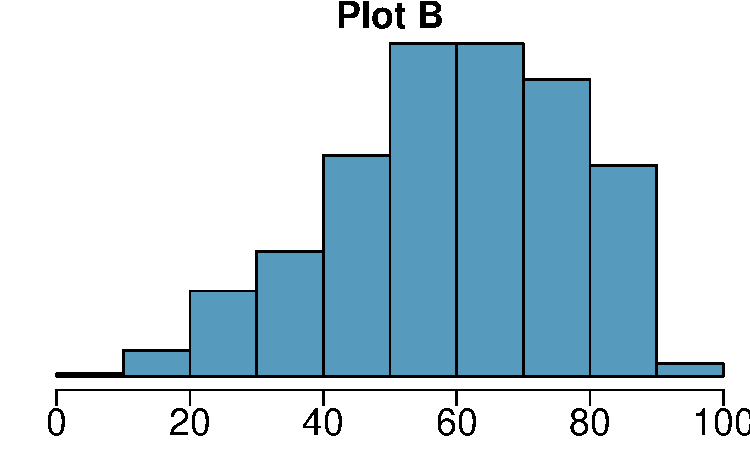
\includegraphics[width=0.32\textwidth]{figures/cltSimLS/cltSimLS_samp}
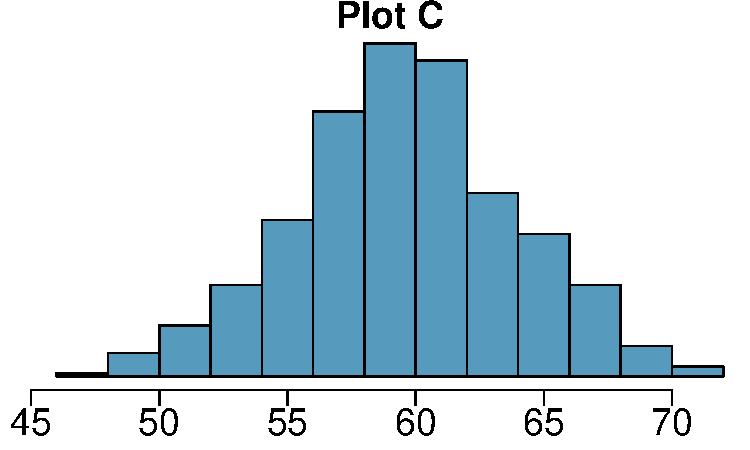
\includegraphics[width=0.32\textwidth]{figures/cltSimLS/cltSimLS_n18}

\end{frame}

%%%%%%%%%%%%%%%%%%%%%%%%%%%%%%%%%%%%

\begin{frame}

\disc{{\small A housing survey was conducted to determine the price of a typical home in Topanga, CA. The mean price of a house was roughly \$1.3 million with a standard deviation of \$300,000. There were no houses listed below \$600,000 but a few houses above \$3 million.}}

\disc{{\small Would you expect most houses in Topanga to cost more or less than \$1.3 million? Hint: What is most likely the shape of this distribution?}}

\pause

\soln{Since the distribution is probably right skewed, the median would be less than the mean, and a majority of observations would be lower than the mean.}


\end{frame}

%%%%%%%%%%%%%%%%%%%%%%%%%%%%%%%%%%%%

\begin{frame}

\disc{{\small A housing survey was conducted to determine the price of a typical home in Topanga, CA. The mean price of a house was roughly \$1.3 million with a standard deviation of \$300,000. There were no houses listed below \$600,000 but a few houses above \$3 million.}}

\clicker{Can we estimate the probability that a randomly chosen house in Topanga costs more than \$1.4 million using the normal distribution?}

\begin{enumerate}[(a)]
\item yes
\item \solnMult{no}
\end{enumerate}

\end{frame}

%%%%%%%%%%%%%%%%%%%%%%%%%%%%%%%%%%%

\begin{frame}

\disc{{\small A housing survey was conducted to determine the price of a typical home in Topanga, CA. The mean price of a house was roughly \$1.3 million with a standard deviation of \$300,000. There were no houses listed below \$600,000 but a few houses above \$3 million.}}

\clicker{Can we estimate the probability that the mean of 60 randomly chosen houses in Topanga is more than \$1.4 million?}

\begin{enumerate}[(a)]
\item \solnMult{yes}
\item no
\end{enumerate}

\end{frame}

%%%%%%%%%%%%%%%%%%%%%%%%%%%%%%%%%%%%

\begin{frame}

\disc{{\small A housing survey was conducted to determine the price of a typical home in Topanga, CA. The mean price of a house was roughly \$1.3 million with a standard deviation of \$300,000. There were no houses listed below \$600,000 but a few houses above \$3 million.}}

\disc{{\small What is the probability that the mean of 60 randomly chosen houses in Topanga is more than \$1.4 million?}}

\pause

In order to calculate $P(\bar{X} > 1.4~mil)$, we need to first determine the distribution of $\bar{X}$. According to the CLT,

\pause

\[ \bar{X} \pause \sim N \pause \left( mean = 1.3, \pause SE = \frac{0.3}{\sqrt{60}} = 0.0387 \right) \]

\pause

\begin{eqnarray*}
P(\bar{X} > 1.4 ) &=& P\left(Z > \frac{1.4 - 1.3}{0.0387}\right) \\
\pause
&=& P(Z > 2.58) \\
\pause
&=& 1 - 0.9951 \pause =  0.0049
\end{eqnarray*}

\end{frame}

%%%%%%%%%%%%%%%%%%%%%%%%%%%%%%%%%%%%

\end{document}